
\section{Analysis}
\subsection{General Assertion of Statistical Error}
The number of decays follows a \person{Poission} distribution due to the
physical and statistical nature of the decay process. Lets assume we measure
$n$ decays in a certain energy range (channel). Then the standard
deviation \cite{cowan} of $n$ is
\begin{align}
  s_n = \sqrt{n}. \label{eq:stddevCounts}
\end{align}
When dealing with different measurement durations $t$ it is more convenient to
compute the event rate $R = \frac{n}{t}$. With \person{Gaussian} error
propagation \cite{cowan} we know that the standard deviation of the event
rate is given by
\begin{align}
  s_R = \frac{s_n}{t} = \frac{\sqrt{n}}{t}. \label{eq:stddevRate}
\end{align}
Here we assumed that the error of the measurement duration $t$ is
neglectable\footnote{In our experiment the measurement duration is given by
the so called \emph{live time} designation of the MCA readout software.}.

\newcommand{\Rmeas}{\ensuremath{R_{\mathrm{meas}}}}
\newcommand{\Rbg}{\ensuremath{R_{\mathrm{bg}}}}
\newcommand{\Rrc}{\ensuremath{R_{\mathrm{rc}}}}

In our analysis we subtract the background event rate $\Rbg =
\frac{n_{\mathrm{bg}}}{t_{\mathrm{bg}}}$ from our measured event rate
$\Rmeas = \frac{n}{t}$. In some cases we even have to subtract the rate of
random coincidences $\Rrc = \frac{n_{\mathrm{rc}}}{t_{\mathrm{rc}}}$ from
our signal, i.e. 
\begin{align}
  R = \Rmeas - \Rbg \quad \textrm{and} \quad R' = \Rmeas - \Rbg - \Rrc.
\end{align}
The standard deviation of the rates on the right sides\footnote{Note that the
random variables \Rmeas, \Rbg  and \Rrc  are statistically independent.} can
be calculated using (\ref{eq:stddevRate}). With \person{Gaussian} error
propagation we can calculate the error of our signal rates $R$ and
$R'$
\begin{align}
  s_R = \sqrt{s_{\Rmeas}^2 + s_{\Rbg}^2} = \sqrt{\frac{n}{t^2} + \frac{n_{\mathrm{bg}}}{t_{\mathrm{bg}}^2}}
  \label{eq:stddevBack}
\end{align}
and
\begin{align}
  s_R = \sqrt{s_{\Rmeas}^2 + s_{\Rbg}^2 + s_{\Rrc}^2} 
      = \sqrt{\frac{n}{t^2} + \frac{n_{\mathrm{bg}}}{t_{\mathrm{bg}}^2} +
      \frac{n_{\mathrm{rc}}}{t_{\mathrm{rc}}^2}}
  \label{eq:stddevRC}
\end{align}

We assume that the standard deviation of the channel $C$ assignment, which
is done by our MCAs, is given by the channel resolution. Therefore 
\begin{align}
  s_C = 1. \label{eq:stddevChannel}
\end{align}

We will use these standard deviations in our plots and fits.


\subsection{Energy Calibration}
\label{sss:calib}
In the background revised decay spectra of \Na and \Cs are certain peaks and
edges with known energies. Further information on the origin of these edges
and peaks can be found in \cite{fluegge}.

The peaks correspond to sharply defined spectral
lines which are broadened by the uncertainty relation (natural line width)
and the \person{Doppler} effect and therefore are a \person{Breit Wigner}
curve. The width in our spectrum depends mainly on
the resolution of our measurement apparatus. The signal we measure is a
convolution of the \person{Breit Wigner} and the resolution function of our
apparatus. The convolution is in good approximation a \person{Gaussian}.
Therefore we fit the peaks with a \person{Gaussian}.

The edges correspond to the \compton edge. The edge could in principal be
described by a Heaviside step function. The signal we measure is again the
convolution of Heaviside step function and resolution function, i.e. the
error function $\mathrm{erf}$. Therefore we fit the \compton edge with an error
function.

\subsubsection{Inorganic Scintillator}
We will now calculate the calibration function of the inorganic scintillator,
the NaI scintillator.

In figure \ref{fig:calibNaJCs} we plotted the background revised event rates
\begin{align}
  R_{\mathrm{NaJ,Cs}} = \Rmeas - \Rbg
\end{align}
 of \Cs and in
figure \ref{fig:calibNaJNa} the background revised event rates
of \Na. The standard deviation is given by (\ref{eq:stddevBack}). In both decay spectra we have fitted the visible peaks and edges. The
$\chi^2/\mathrm{ndf}$ is always between $0.9$ and $1.3$ which means that the
assumptions of the fit function are good.
\begin{figure}[tbp]
  \centering
  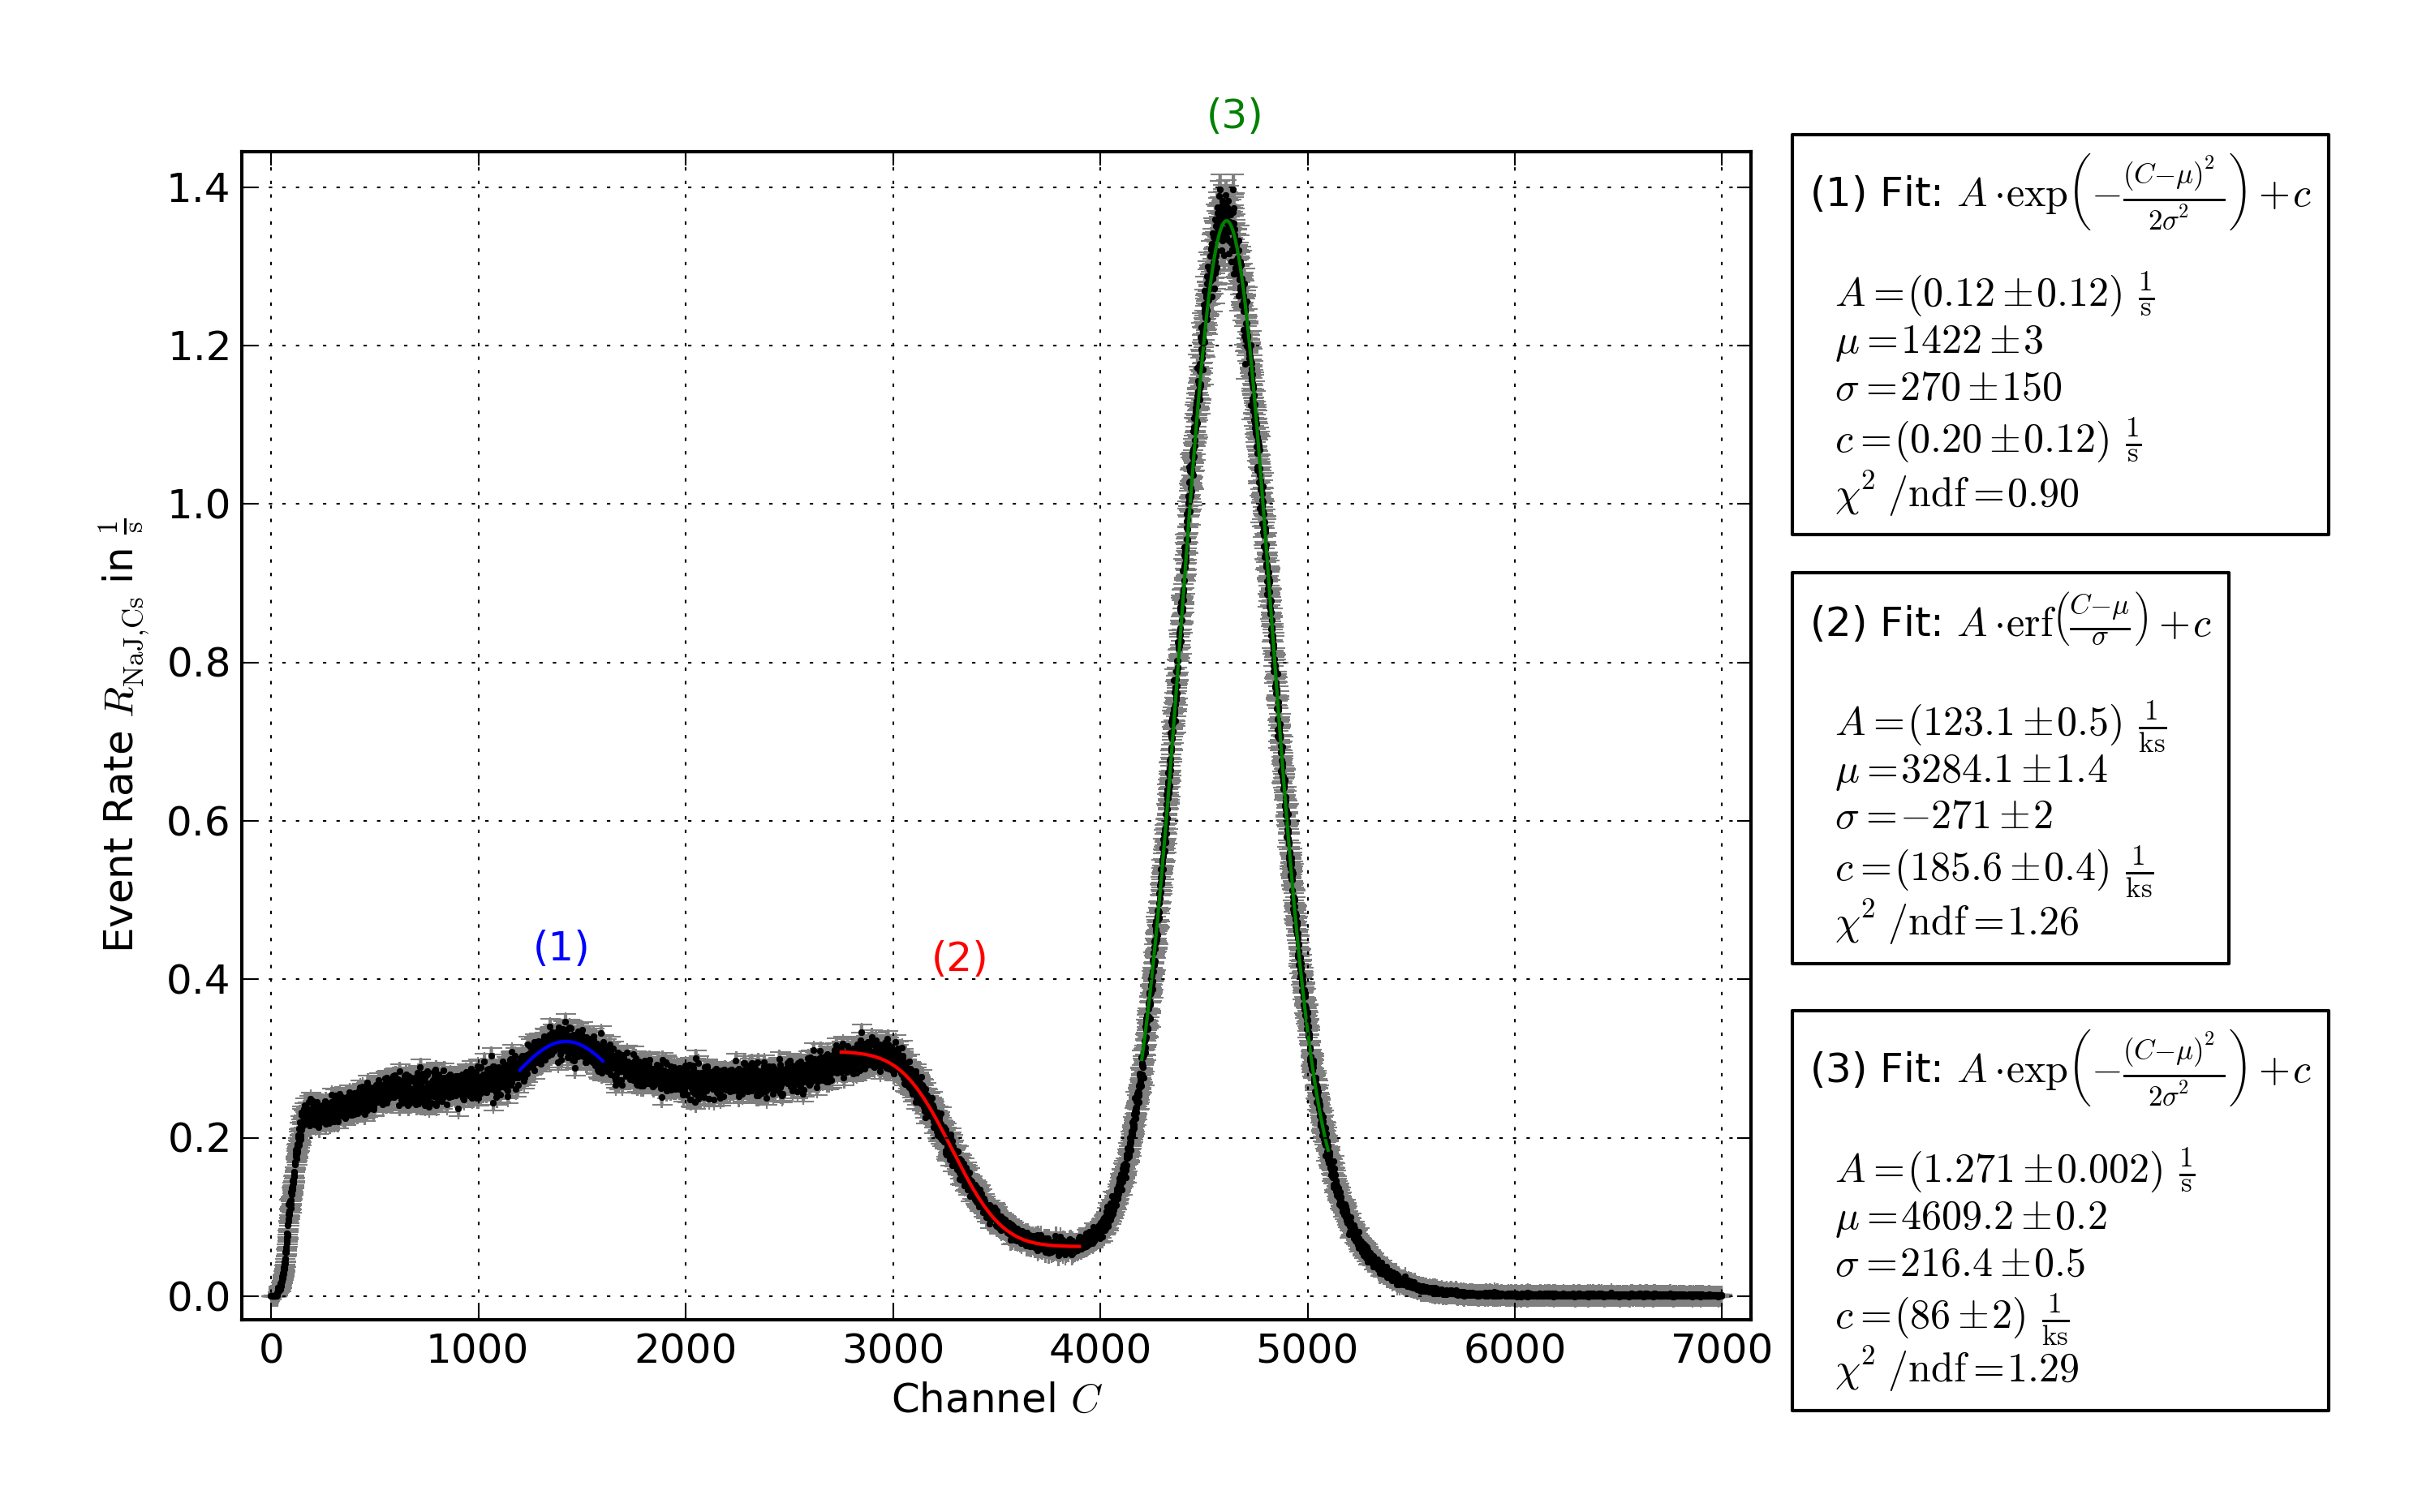
\includegraphics[width=1.0\textwidth]{plots/naj_cs.png}
  \caption{Background revised decay spectrum of \Cs measured with the NaI
  scintillator. Certain peaks and edges are fitted with the corresponding
  function. The gray area corresponds to the error bars. Measurement
  duration $t=3600\mathrm{s}$.}
  \label{fig:calibNaJCs}
\end{figure}

In Table \ref{tab:assignmentNaJ} we have made an assignment of the fitted
channels and the known corresponding energies \cite{anleitung}.

\begin{table}[htb]
  \centering
  \begin{tabular}{rclcl}
  Source & Energy in $\mathrm{keV}$ & Type & Fit \# & Channel $C$
  \\\toprule[1.5pt]
  \Cs & 183 & back scattering edge & 1 & $\pyexp{calib_naj_cs_1}$\\ 
   & 477 & \compton edge & 2 & $\pyexp{calib_naj_cs_2}$\\ 
   & 662 & spectral line & 3 & $\pyexp{calib_naj_cs_3}$\vspace{0.3em}\\
  \Na & 341 & \compton edge & 1 &  $\pyexp{calib_naj_na_1}$\\ 
   & 511 & annihilation of $e^+$ and $e^-$ & 2 &  $\pyexp{calib_naj_na_2}$\\
   & 1064 & \compton edge & 3 &  $\pyexp{calib_naj_na_3}$\\ 
   & 1277 & spectral line & 4 &  $\pyexp{calib_naj_na_4}$\\\bottomrule[1.5pt]
  \end{tabular}
  \caption{Assignment of fitted peaks and edges to the known energies
  \cite{anleitung} for the NaJ scintillator.}
  \label{tab:assignmentNaJ}
\end{table}

We can now plot the energy channel pairs for the NaI scintillator, see
figure \ref{fig:calibNaJ}. The relation between channel and energy should be
a first order polynomial.
\begin{align}
  E(C) = a + b \cdot C \label{eq:ec_eq}
\end{align}
But the data points do not lay on the fit within their standard deviation
what causes a very large $\chi^2/\mathrm{ndf} = 40$. This might be caused
by unknown/untreated uncertainties, which would have enlarged the standard
deviation, or by more complex effects in the scintillator, so that a higher
polynomial is needed.

\begin{figure}[tbp]
  \centering
  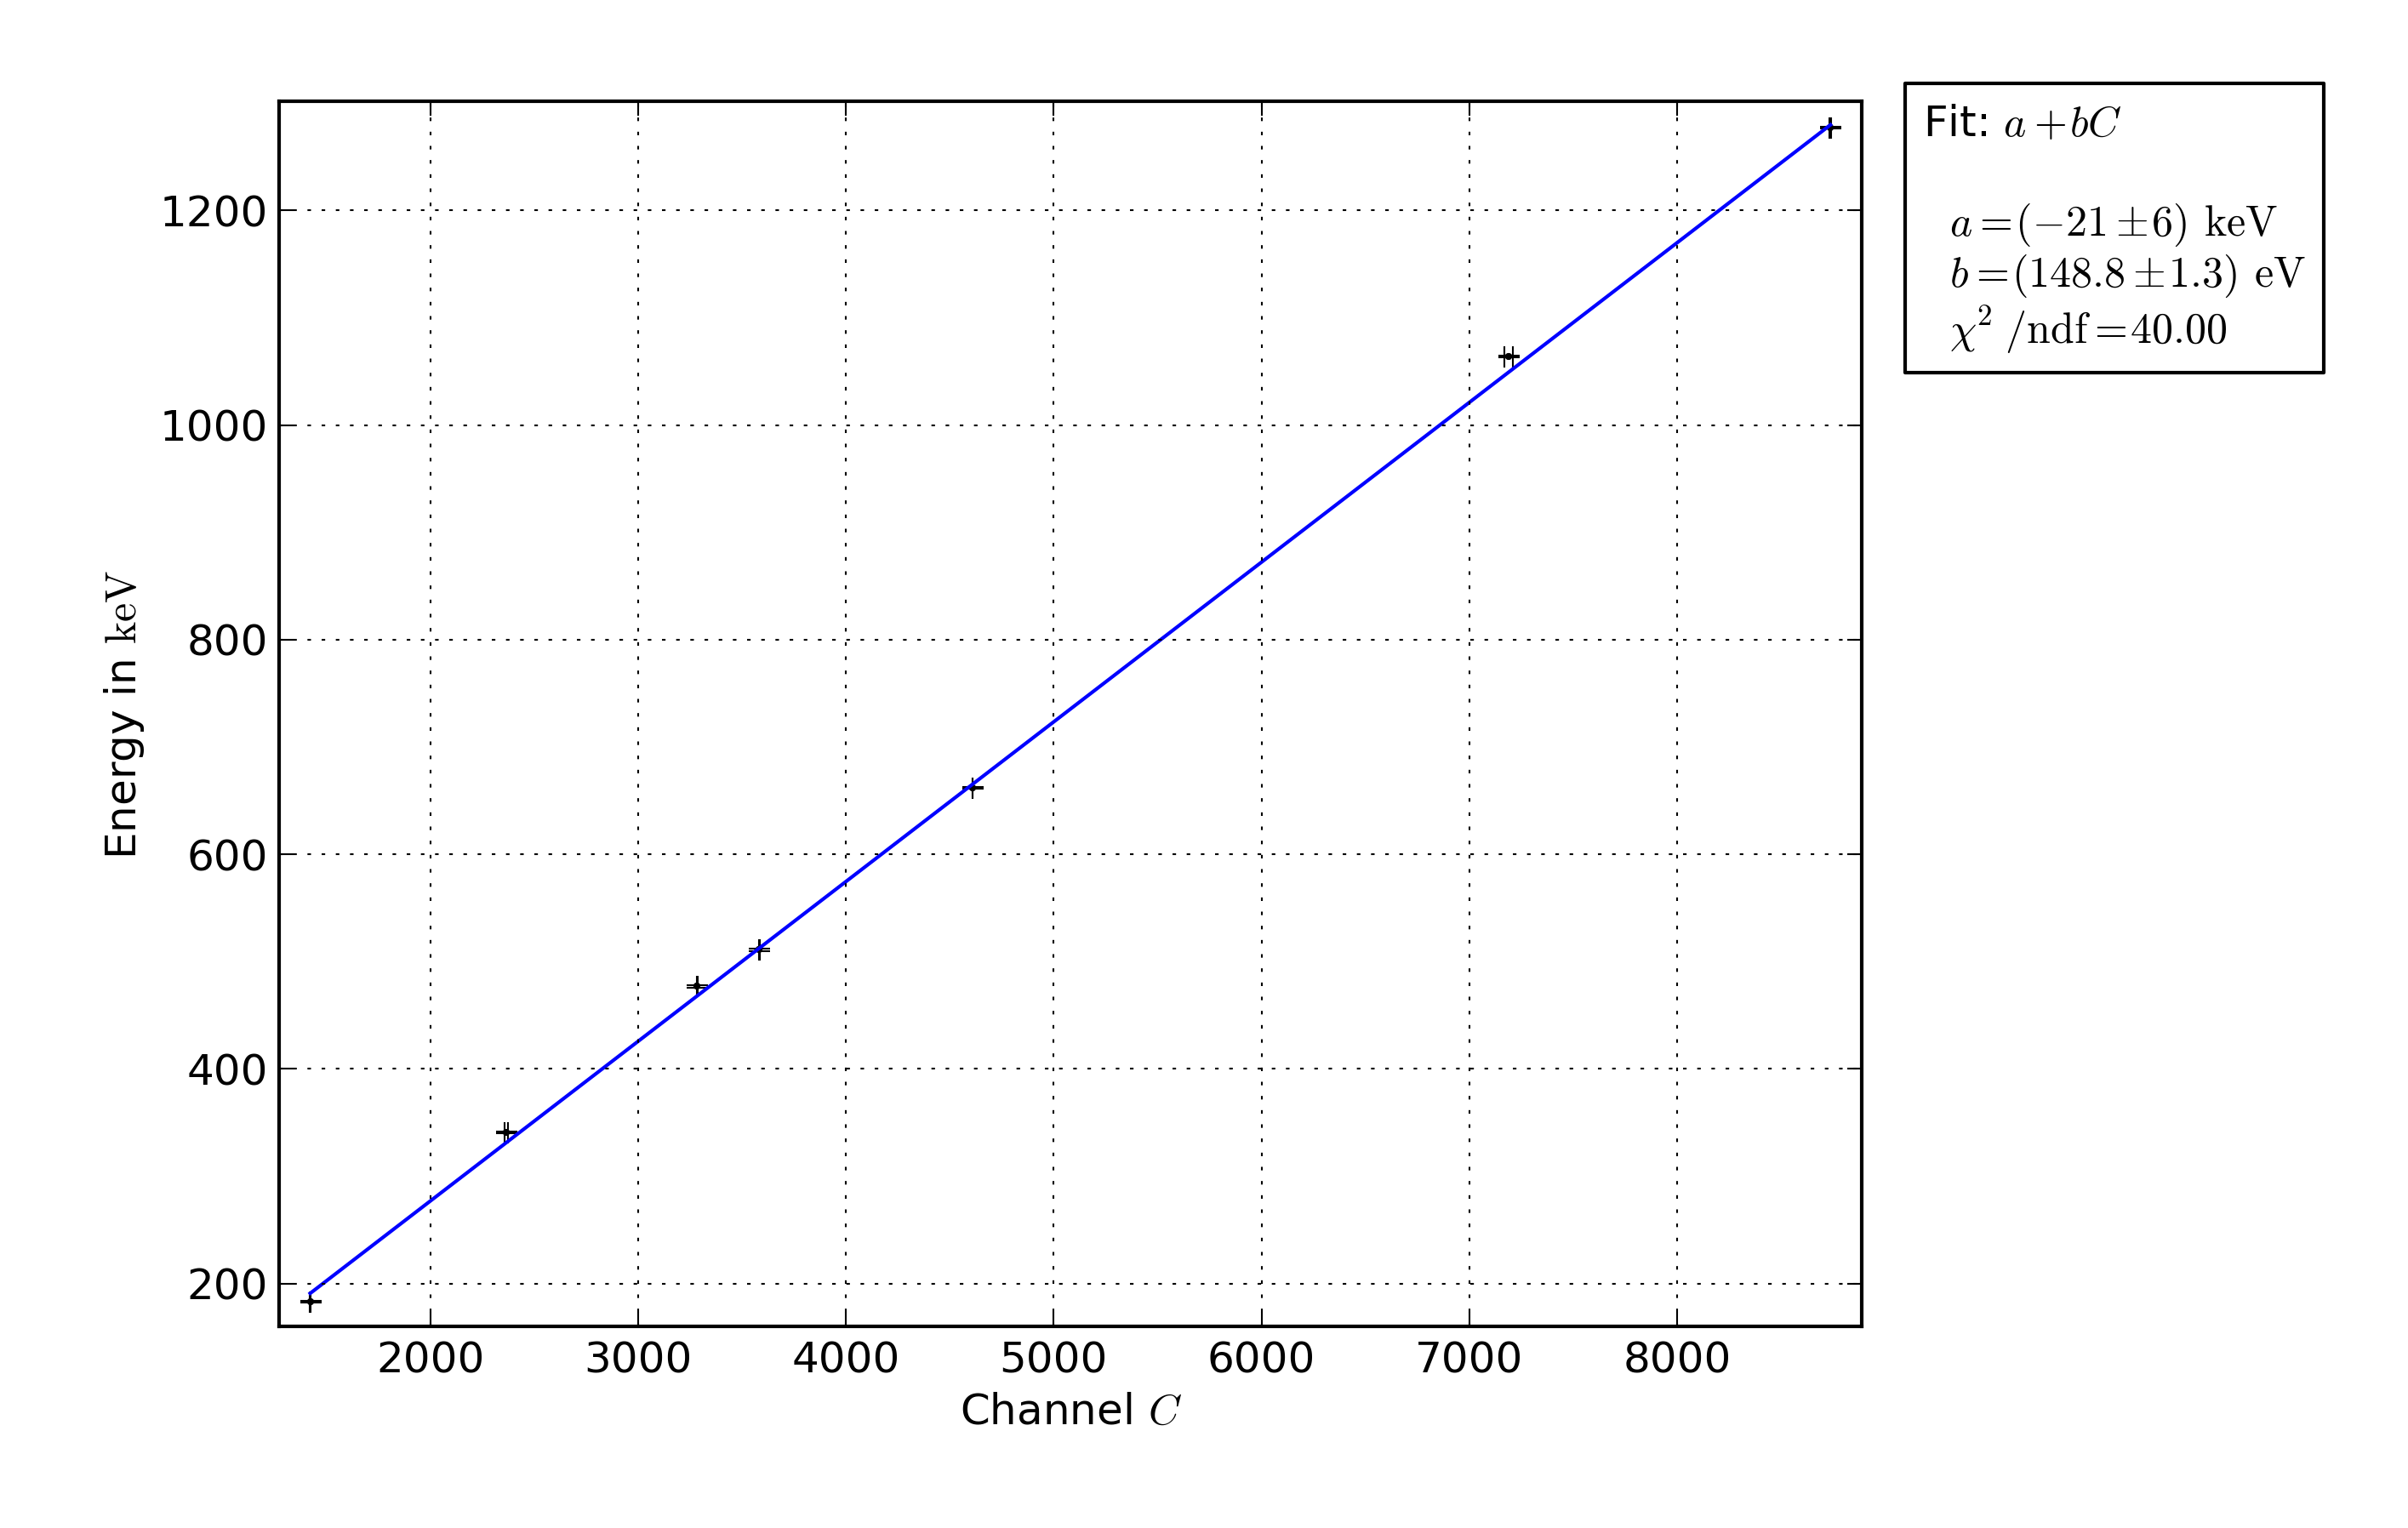
\includegraphics[width=1.0\textwidth]{plots/calib_naj.png}
  \caption{Energy-Channel pairs and fit for NaI scintillator. The values are
  taken from table \ref{tab:assignmentNaJ}. The $x$-error bars are taken
  from the fit results.  The $y$-errors are assumed to be $s_E =
  1\mathrm{keV}$.}
   \label{fig:calibNaJ}
\end{figure}

Anyway, the fitted calibration function (\ref{eq:ec_eq}) for the NaJ
scintillator is
\begin{align}
  E_{\mathrm{NaI}}(C) = \pyexp{calib_naj_a} + \pyexp{calib_naj_b} \cdot C.
  \label{eq:calib_naj}
\end{align}

\subsubsection{Organic Scintillator}
We have to do the same calibration as we did with the inorganic
scintillator. The corresponding spectra (figure \ref{fig:calibPVCCs} and
\ref{fig:calibPVCNa}) and the assignments (table \ref{tab:assignmentPVC}) can be
found in the appendix.

In this case we only have three known energy channel pairs, which are shown
in figure \ref{fig:calibPVC}.  We have fitted the same linear function
(\ref{eq:ec_eq}). The resulting calibration function is
\begin{align}
  E_{\mathrm{PVC}}(C) = \pyexp{calib_pvc_a} + \pyexp{calib_pvc_b} \cdot C.
  \label{eq:calib_pvc}
\end{align}

\begin{figure}[tbp]
  \centering
  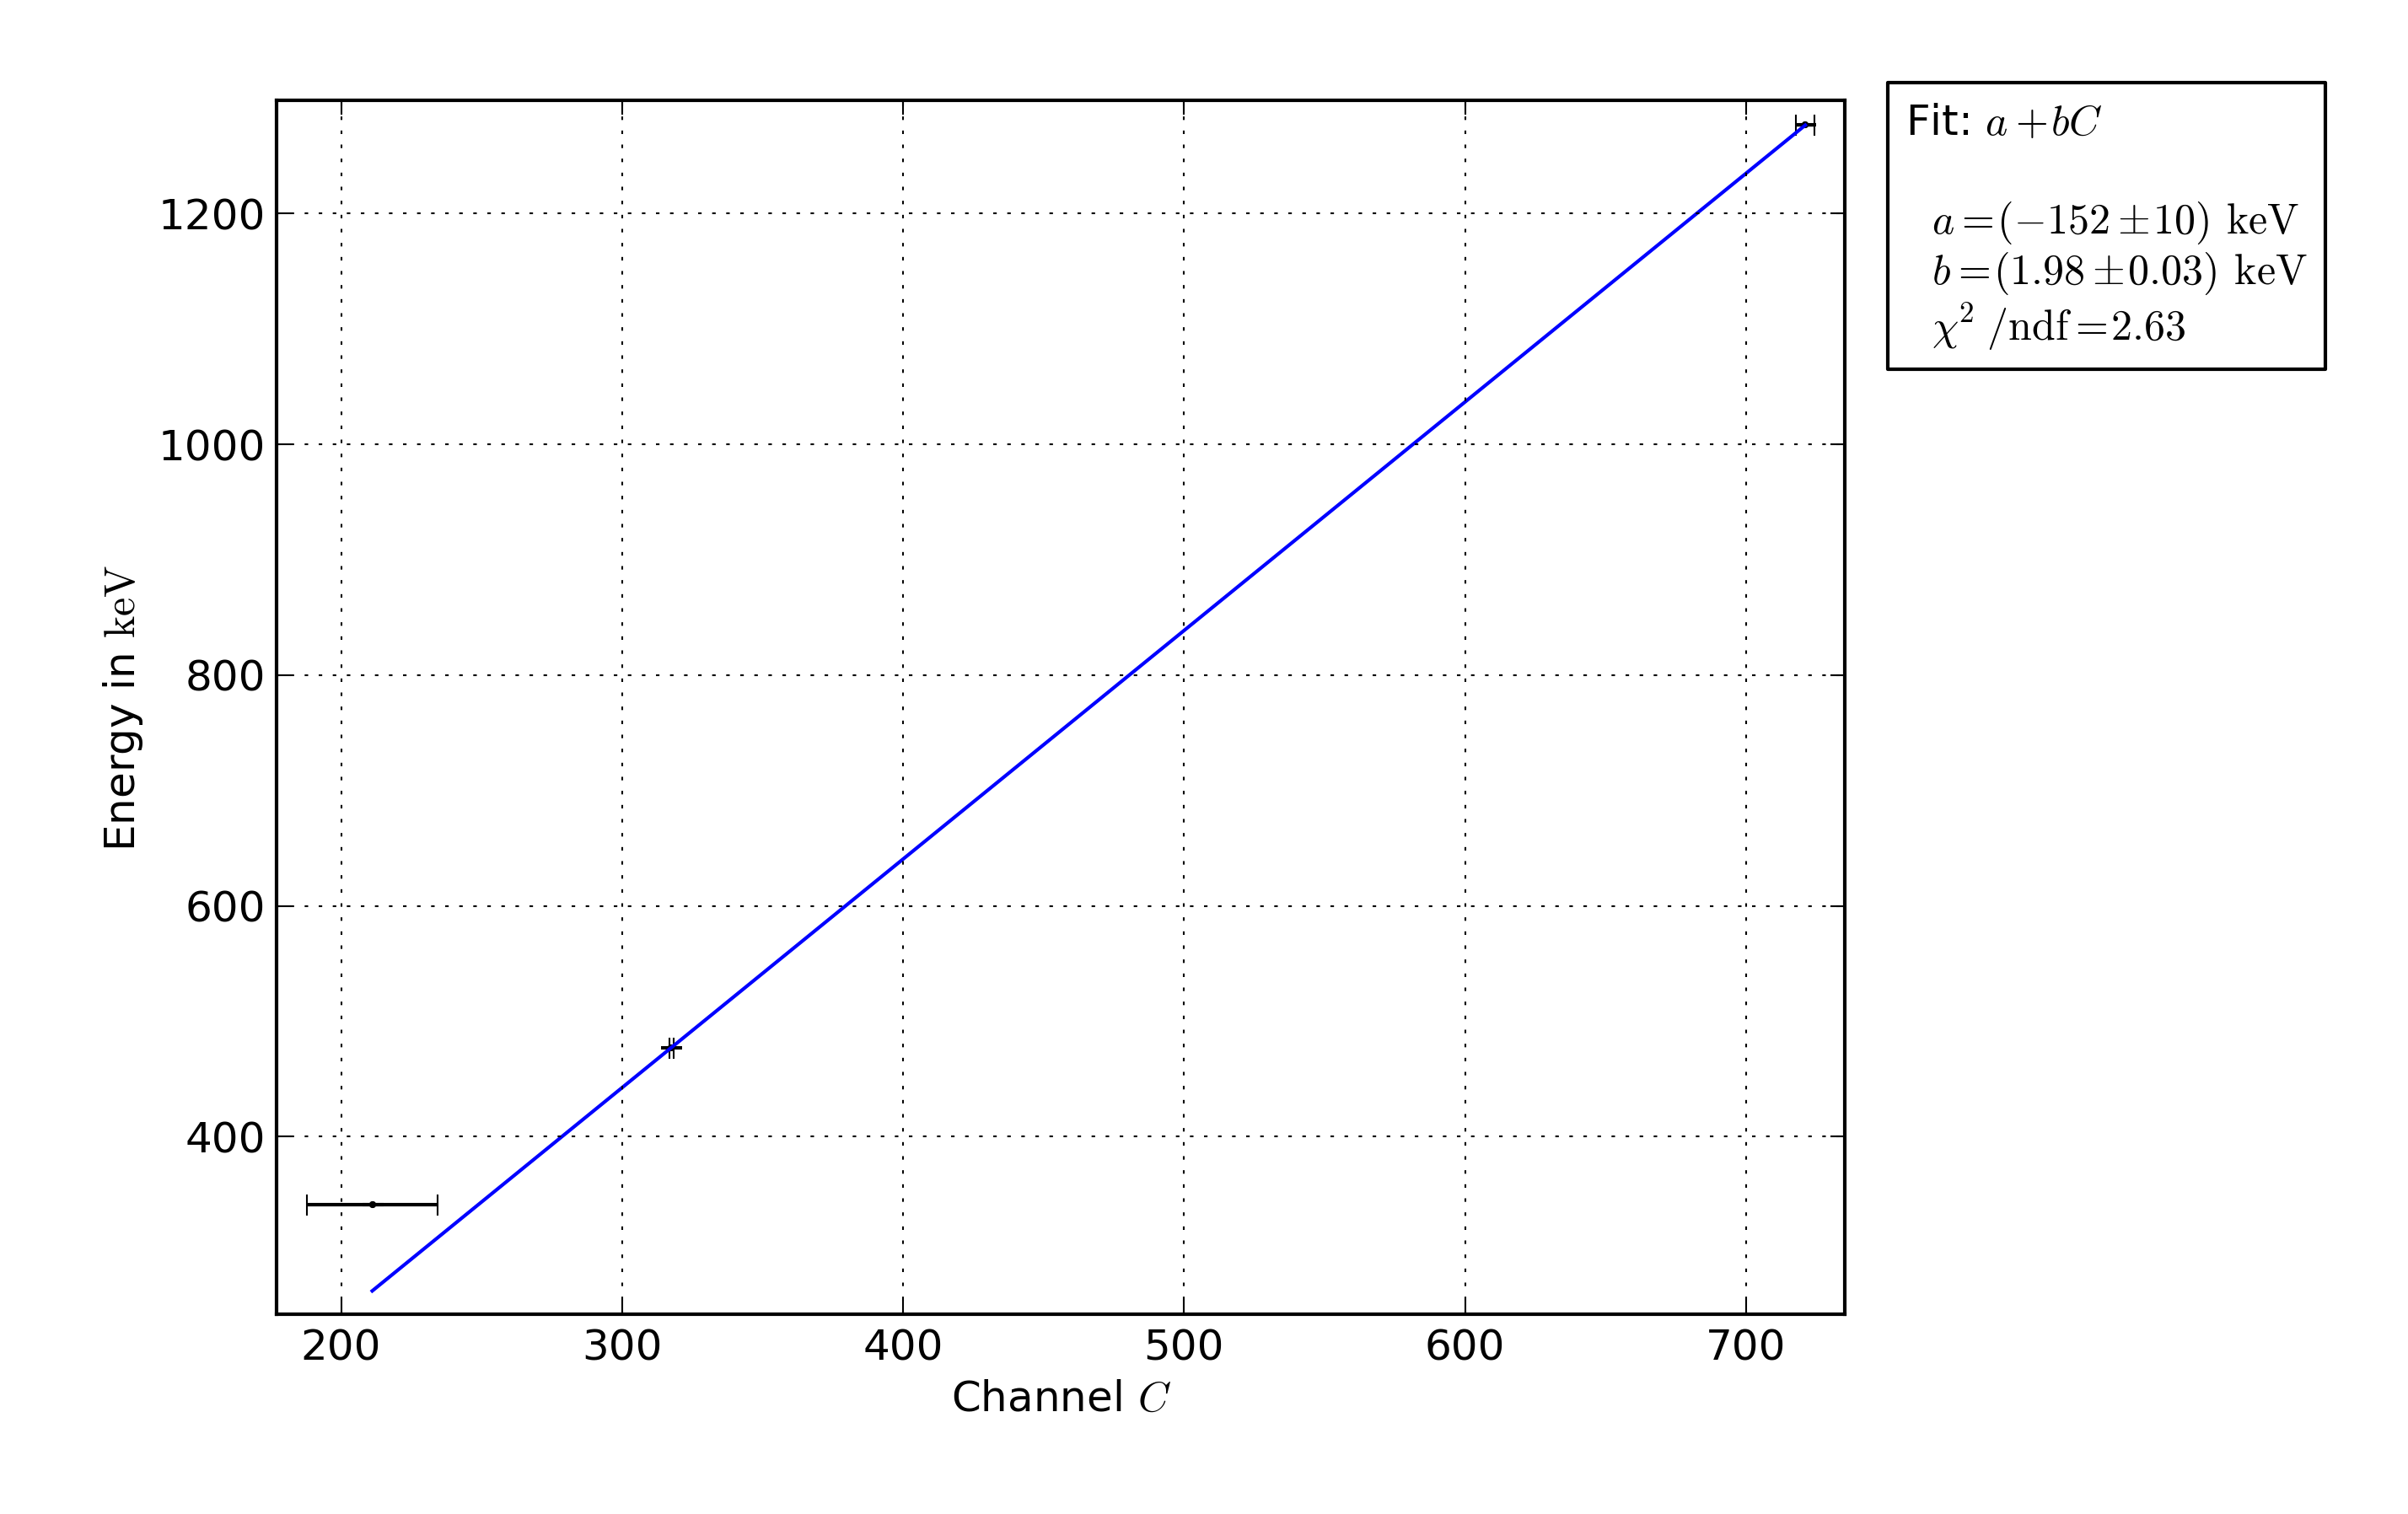
\includegraphics[width=1.0\textwidth]{plots/calib_pvc.png}
  \caption{Energy-Channel pairs and fit for PVC scintillator. The values are
  taken from table \ref{tab:assignmentPVC}. The $x$-error bars are taken
  from the fit results.  The $y$-errors are assumed to be $s_E =
  1\mathrm{keV}$.}
   \label{fig:calibPVC}
\end{figure}


\FloatBarrier
\subsection{Conservation of Energy}
In the derivation of the elastic \compton scattering we have used the law of
conservation of total energy, see (\ref{eq:csDerivation1}). Now we want to
verify this assumption experimentally.

We have subtracted the background and the random coincidences from the
recorded spectra of both scintillator and for various angles $\theta$
\begin{align}
  R = \Rmeas - \Rbg - \Rrc.
\end{align}
Here the error propagation (\ref{eq:stddevRC}) applies. One of these revised
spectra is exemplarily shown in figure \ref{fig:conserv45_}.
\begin{figure}[h!]
  \centering
  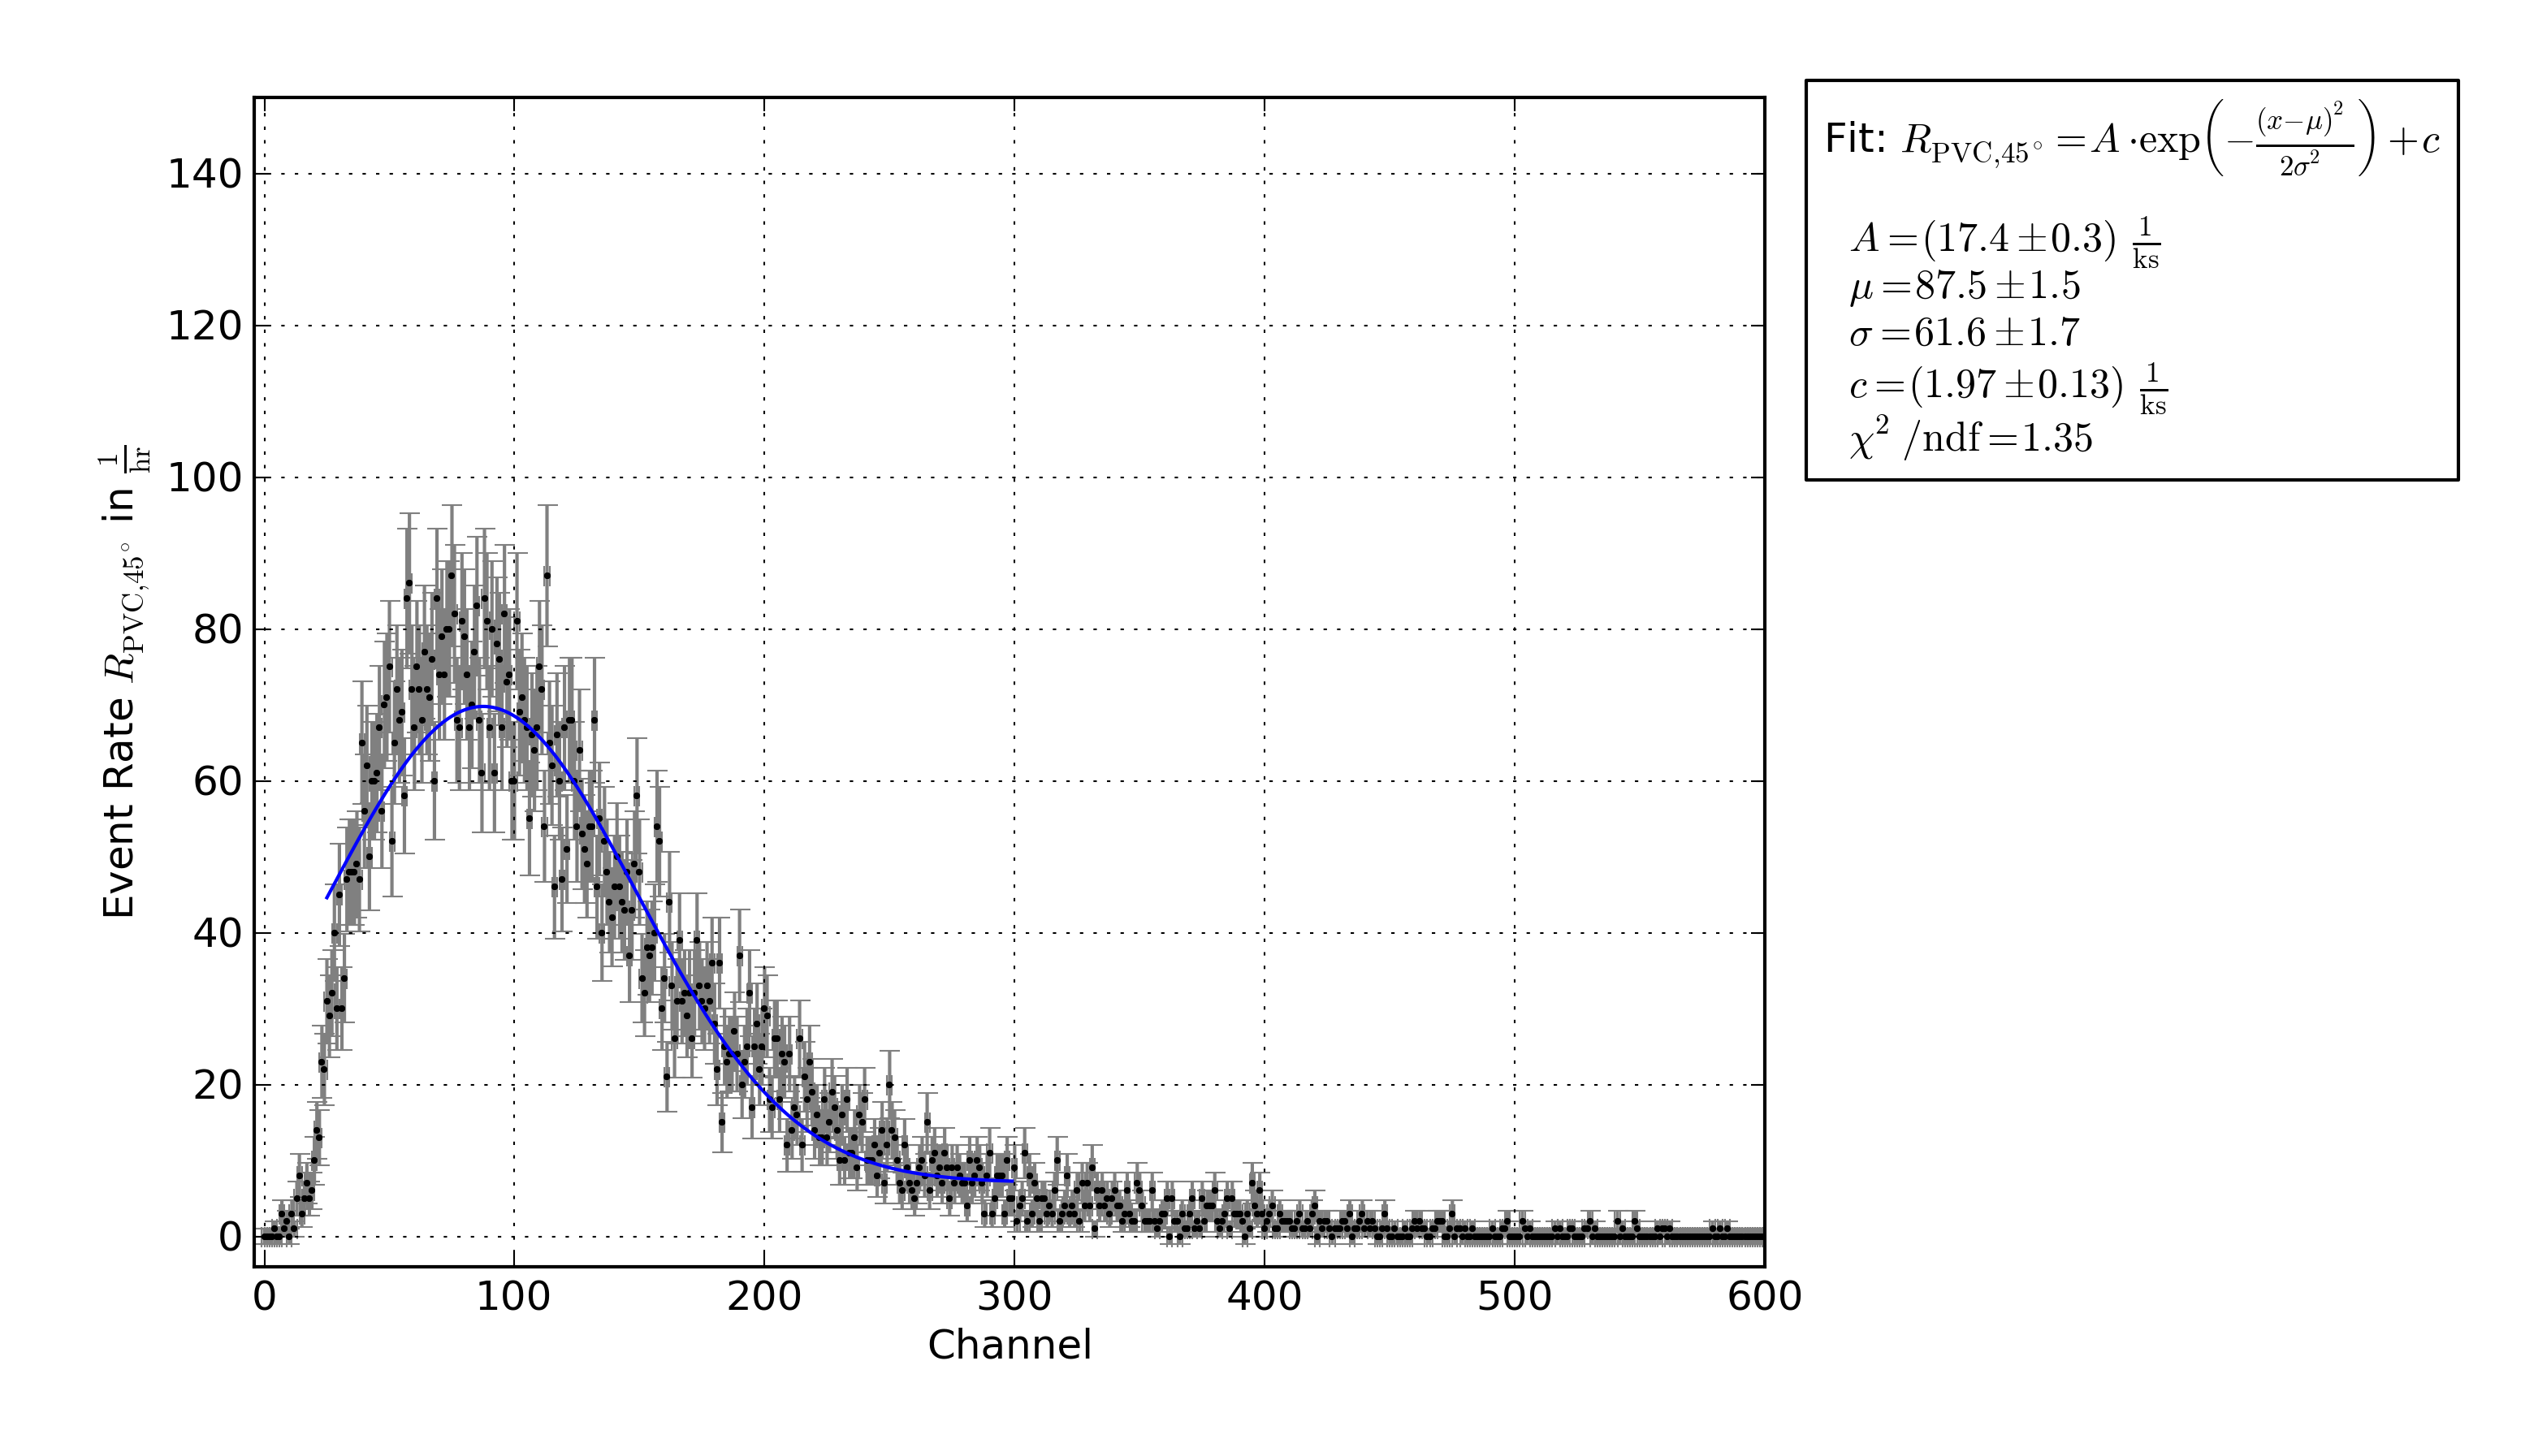
\includegraphics[width=\textwidth]{plots/pvc_45.png}
  \caption{Electron energy spectrum (PVC scintillator) of coincident signals
  with $\theta=45\degree$.}
  \label{fig:conserv45_}
\end{figure}

We have fitted the peaks of the scattered electrons (PVC scintillator) and
the peaks of the scattered photons (NaI scintillator) with a
\person{Gaussian}. The fits can be found in the appendix, see figure
\ref{fig:pvc0} through \ref{fig:naj120}. The fit results and the corresponding energies are listed in table
\ref{tab:conserv}. Here we have used the calibration function for each scintillator to calculate the energies.
The standard deviation of the calculated energies can be derived using \person{Gaussian} error propagation
\begin{align}
  s_E = \sqrt{s_a^2 + C^2 s_b^2 + b^2 s_C^2}
\end{align}
where $a$ and $b$ are the calibration fit parameters from (\ref{eq:ec_eq}).

\begin{table}[htbp]
  \centering
  \begin{tabular}{r|ll|ll}
   $\theta/\degree$ & Channel $C_{\mathrm{PVC}}$ & $e^-$-Energy $E'_e$ & Channel $C_{\mathrm{NaJ}}$ & $\gamma$-Energy $E'_{\gamma}$ \\ \toprule[1.5pt]
  0 & $\pyexp{pvcC0}$ & $\pyexp{pvcE0}$ & $\pyexp{najC0}$ & $\pyexp{najE0}$ \\ 
  15 & $\pyexp{pvcC15}$ & $\pyexp{pvcE15}$ & $\pyexp{najC15}$ & $\pyexp{najE15}$ \\ 
  30 & $\pyexp{pvcC30}$ & $\pyexp{pvcE30}$ & $\pyexp{najC30}$ & $\pyexp{najE30}$ \\ 
  45 & $\pyexp{pvcC45}$ & $\pyexp{pvcE45}$ & $\pyexp{najC45}$ & $\pyexp{najE45}$ \\ 
  60 & $\pyexp{pvcC60}$ & $\pyexp{pvcE60}$ & $\pyexp{najC60}$ & $\pyexp{najE60}$ \\ 
  75 & $\pyexp{pvcC75}$ & $\pyexp{pvcE75}$ & $\pyexp{najC75}$ & $\pyexp{najE75}$ \\ 
  90 & $\pyexp{pvcC90}$ & $\pyexp{pvcE90}$ & $\pyexp{najC90}$ & $\pyexp{najE90}$ \\ 
  105 & $\pyexp{pvcC105}$ & $\pyexp{pvcE105}$ & $\pyexp{najC105}$ & $\pyexp{najE105}$ \\ 
  120 & $\pyexp{pvcC120}$ & $\pyexp{pvcE120}$ & $\pyexp{najC120}$ & $\pyexp{najE120}$ \\ \bottomrule[1.5pt]
  \end{tabular}
  \caption{Fit results of coincident photon and electron spectrum. The energies were calculated using the calibration functions (\ref{eq:calib_pvc}) and
  (\ref{eq:calib_naj}).}
  \label{tab:conserv}
\end{table}

In figure \ref{fig:conserv}  we have plotted all the energies of the
electron and the photon for different angles. The figure also includes the
sum of both energies and the theoretically expected curves (\ref{eq:egamma})
and (\ref{eq:eelectron}). 


\begin{figure}[h!]
  \centering
  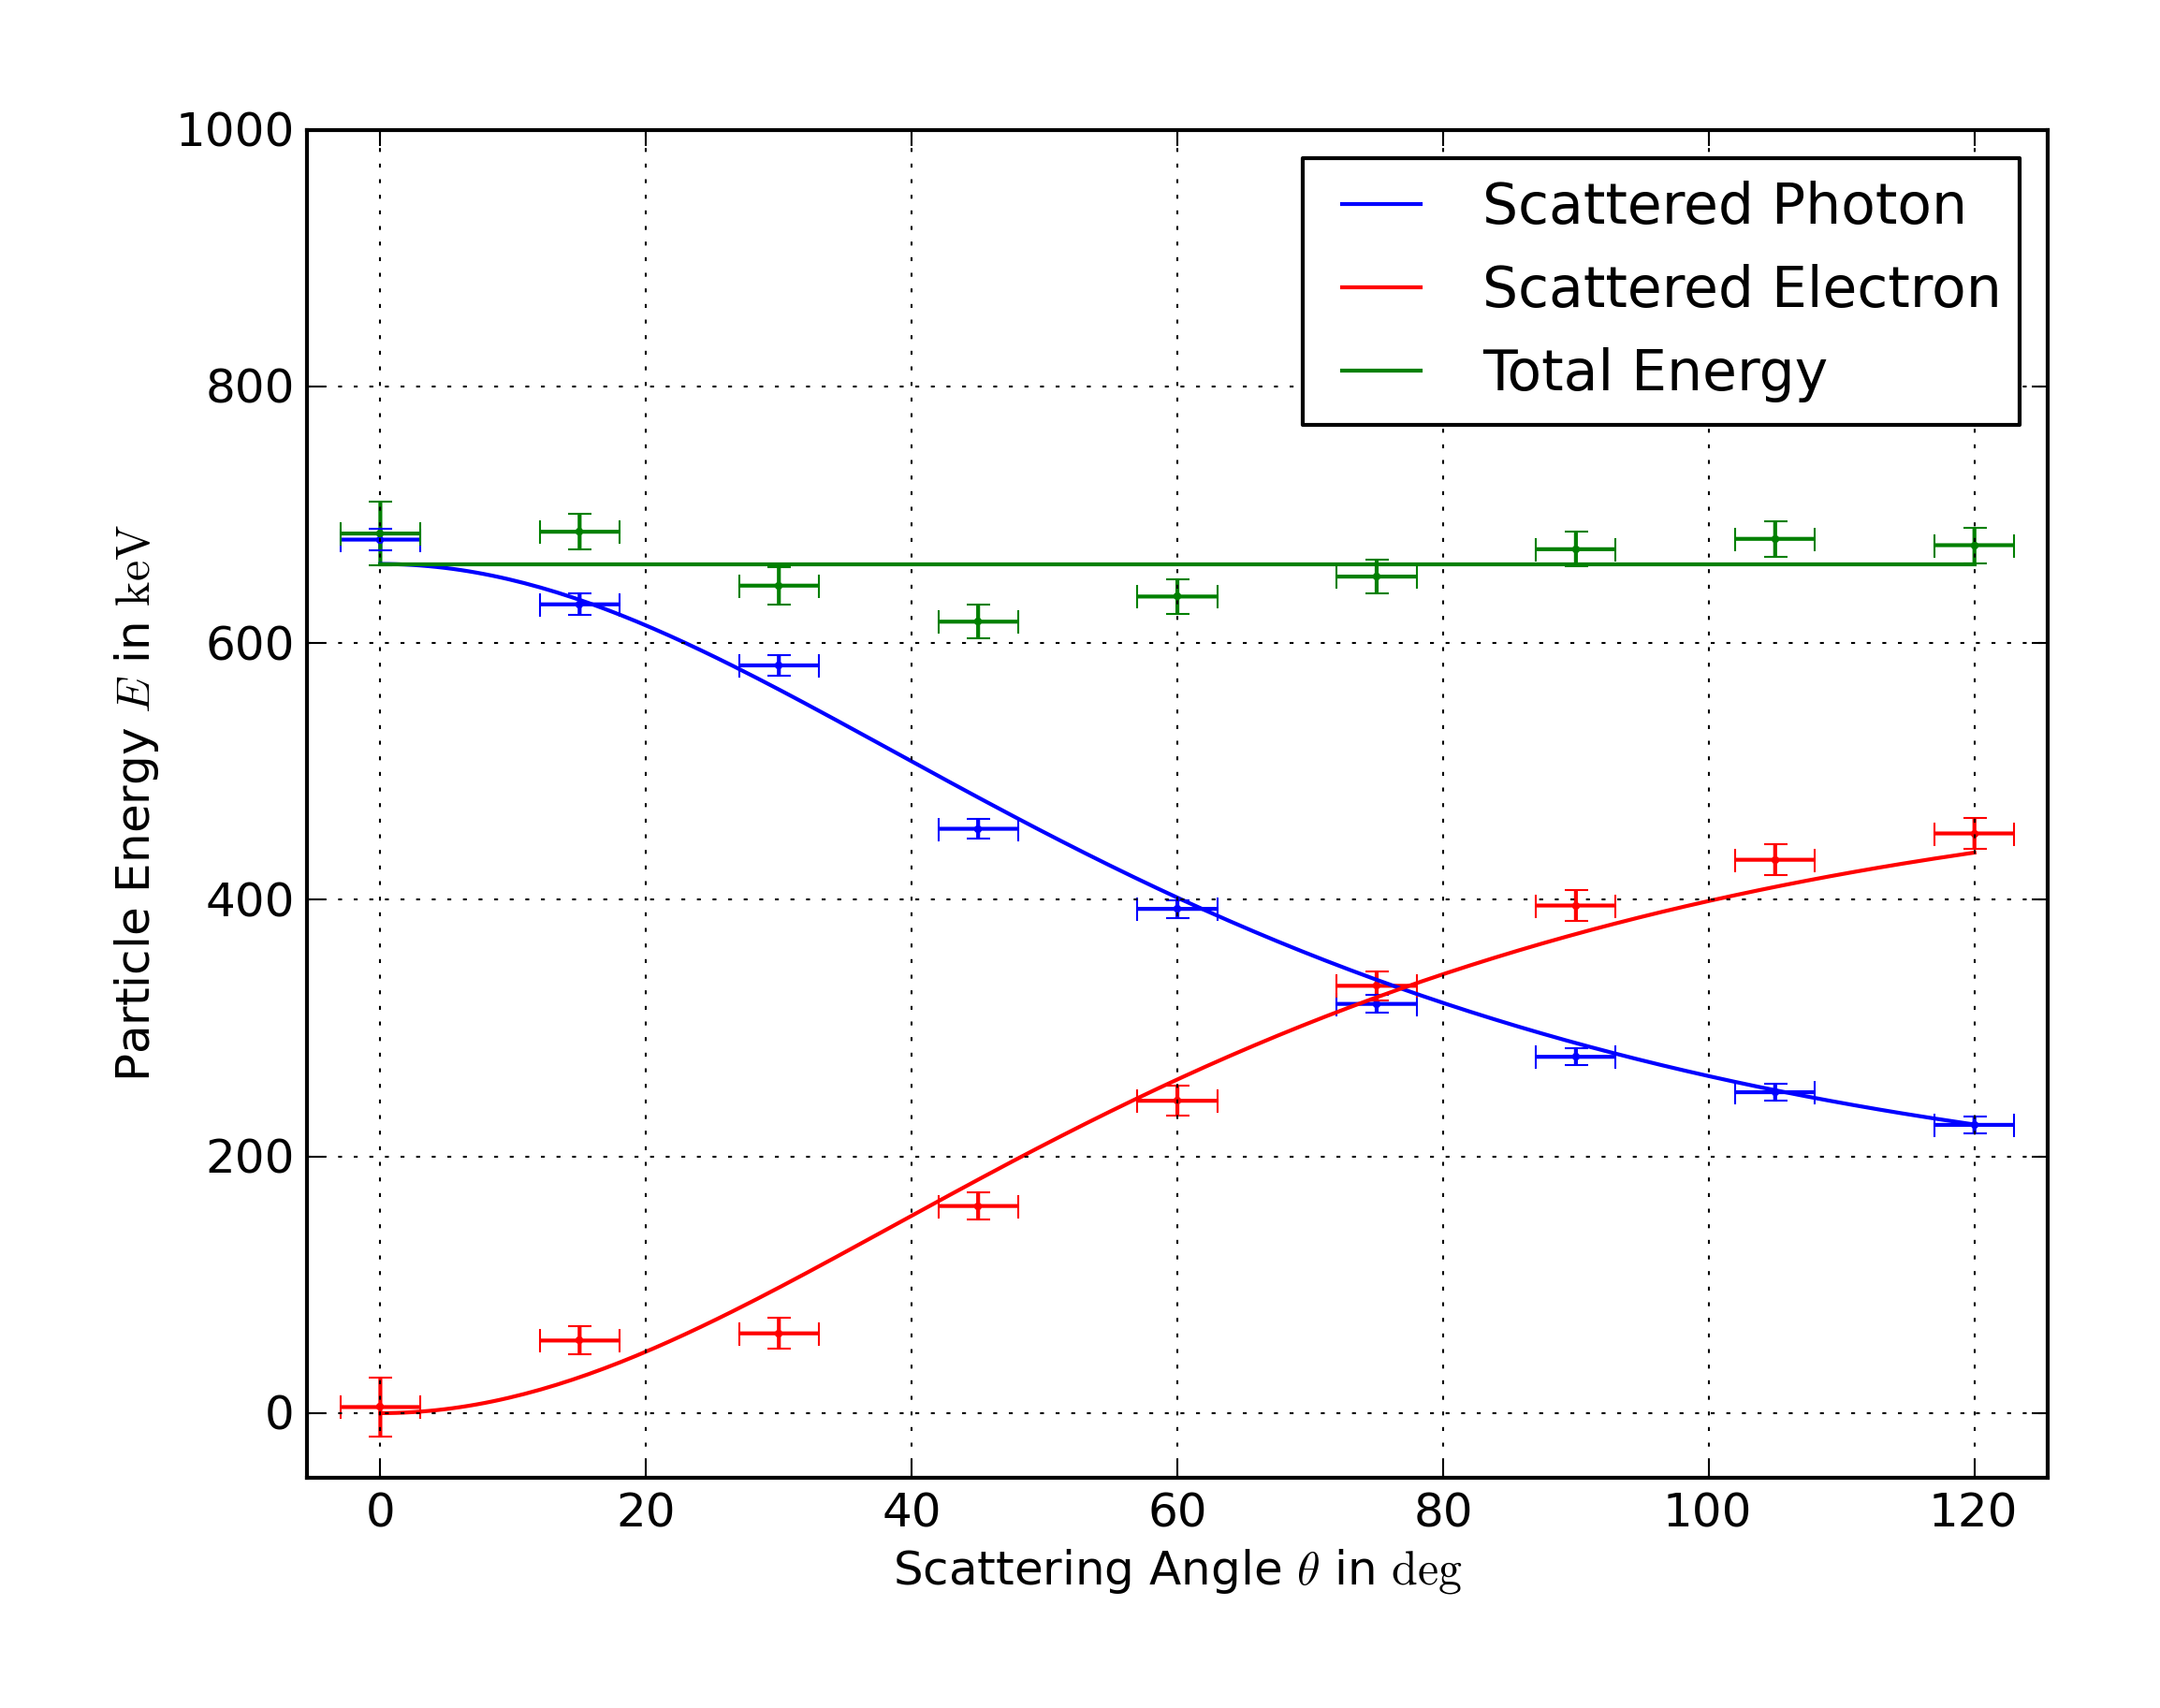
\includegraphics[width=\textwidth]{plots/conservation.png}
  \caption{Measured energies of electron and photon for different angles. The values are taken from table \ref{tab:conserv}. We estimated the standard deviation
  of the angle $s_\theta = 3\degree$. }
  \label{fig:conserv}
\end{figure}

Form figure \ref{fig:conserv} we can say that the sum of the energies is in
agreement with the theoretical constant energy within the standard
deviations. Therefore we verified the conservation of energy in our
measurement. 
\label{sss:conserv}

\FloatBarrier
\subsection{Differential Cross Section}
The differential cross section $\tder{\sigma}{\Omega}$ is given by the
\person{Klein-Nishina} relation (\ref{eq:kleinn}). To calculate the
differential cross section from our measurement we have to determine the
photon intensity $I(\theta)$ at a
certain angle. The peaks of the scattered
photons vary in width, compare figure \ref{fig:naj30} and \ref{fig:naj120}.
The cause might be that the apparatus resolution function is not constant
over the whole energy range. An other cause is the shape of the PVC
scintillator. For small measurement angles the photons can be scatter at the
edge of the
scintillator or in the center. Electrons at the edge have a different
scattering angle compared to the ones scatter in the center. In contrast for
large
measurement angles the side view of the PVC scintillator is less wide, so
that the scattering angle varies less. To account to this, we define the photon
intensity
proportional to the integral over the fitted \person{Gaussian} $A \cdot \exp
\left(-\half \frac{(x-\mu)^2}{\sigma^2}\right)$. We define photon
intensities as
\begin{align}
  I = A \cdot \sigma.
\end{align}
with its standard deviation
\begin{align}
  s_I = \sqrt{A^2 s_\sigma^2 + \sigma^2 s_A^2}.
\end{align}
$A$ and $\sigma$ are the parameters of the \person{Gaussian} fits to the
background and random coincidence revised spectra form \ref{sss:conserv}.

The differential cross section should resemble the probability that the
photon is scattered under an angle of $\theta$.  The probability can be
estimated by the ratio $I(\theta) / I_{\mathrm{in}}$, where $I(\theta)$ is
the photon intensity scattered under an angle of $\theta$ and
$I_{\mathrm{in}}$ is the total photon intensity emitted by the \Cs source.
From our direct intensity measurement (see figure \ref{fig:directI}) we get
$I_{\mathrm{in}} = \pyexp{intensity}$. Furthermore we have to account to the
number $N$ of electrons or the electron density $n_e$. The probability of an
electron being scattered is equal to the ratio of total cross section $N
\cdot \sigma$ and irradiated area $A$ of the scintillator\footnote{ Here we
have made the assumption that the cross sections of all electrons do not
overlap. Depending on the thickness of the scintillator, this might not be
correct.}, see figure \ref{fig:crossDer}.
\begin{align}
  \frac{\sigma N}{A} &= \frac{I}{I_{\mathrm{in}}} \\
 \Leftrightarrow\quad \sigma &= \frac{I}{I_{\mathrm{in}}} \frac{A}{N} = 
    \frac{I}{I_{\mathrm{in}}} \frac{1}{\frac{N}{A d} d} \overset{Ad=V}{=}
    \frac{I}{I_{\mathrm{in}}} \frac{1}{n_e d}
    \label{eq:predcs}
\end{align}
\begin{figure}[h!]
  \centering
  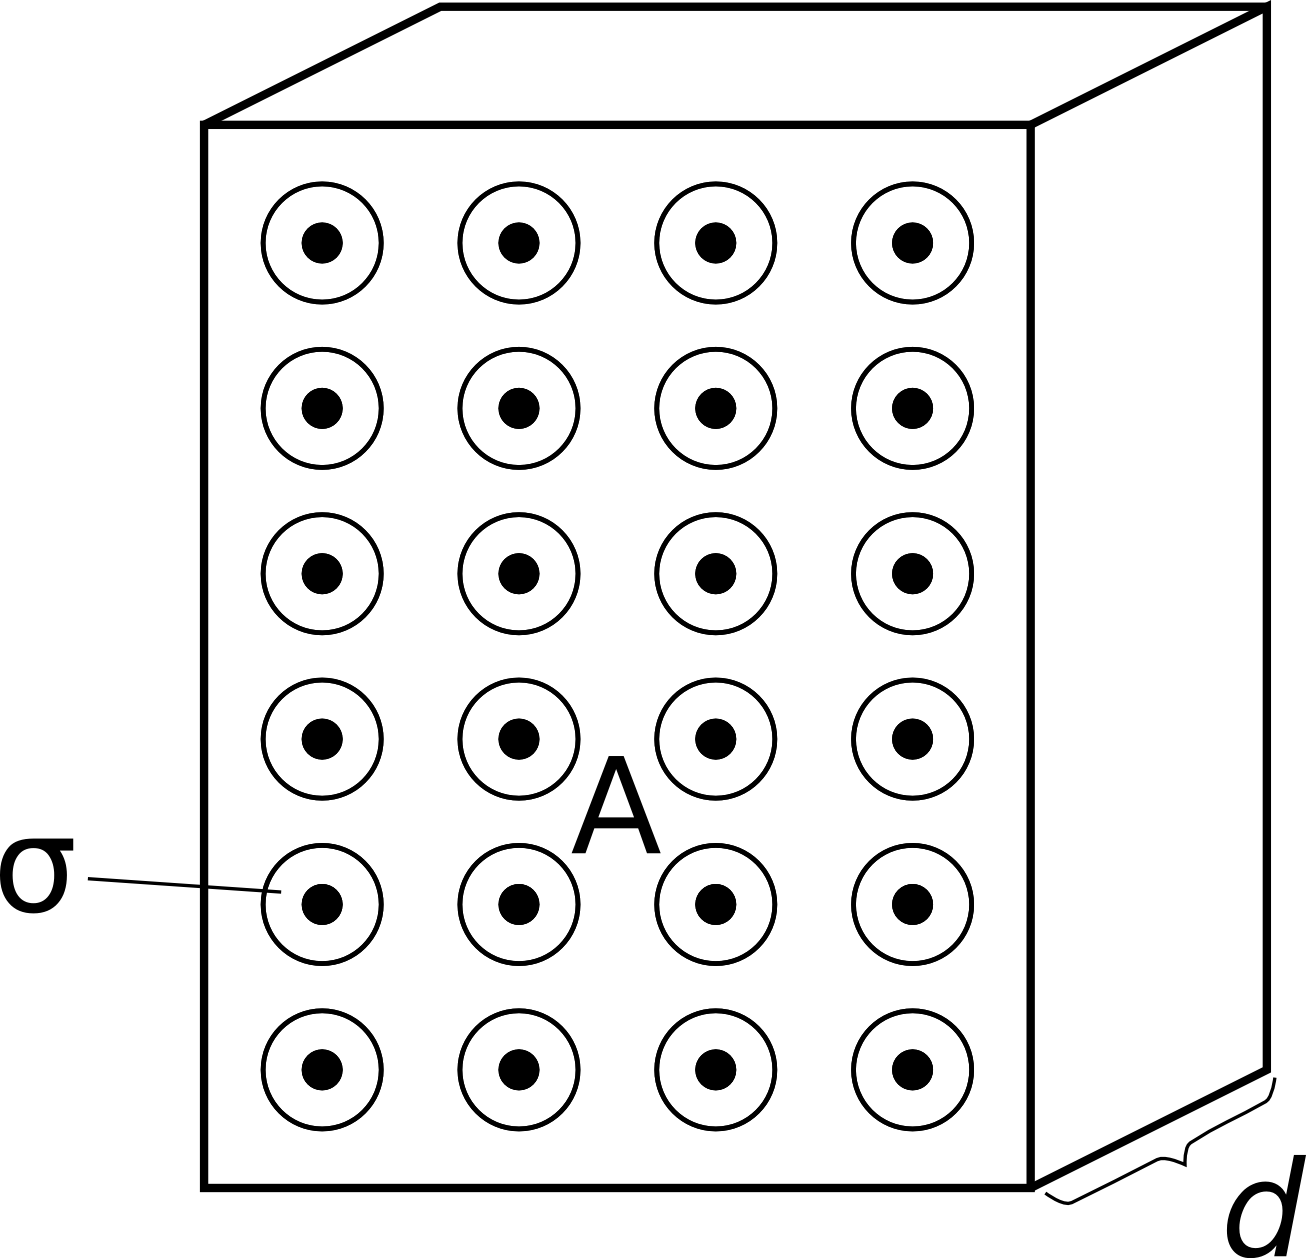
\includegraphics[width=0.35\textwidth]{cross.png}
  \caption{Illustration of the cross section (geometrical interpretation). The
  bock represents the PVC scintillator. $A$ is the irradiated area of the
  scintillator and $d$ its thickness. The back dots represent electrons and the
  circles around it represent the cross section $\sigma$.}
  \label{fig:crossDer}
\end{figure}

To get the \emph{differential} cross section, we have to derivate
(\ref{eq:predcs}) with respect to the solid angle $\Omega$. In our experiment we have measured the averaged
spherical intensity, due to the finite dimensions of the NaI scintillator
\begin{align}
  I = \oneover{\Ddif{\Omega}} \int_{\Omega_0}^{\Omega_1} \tdif{\Omega} I(\Omega).
\end{align}
where the NaI scintillator covers the solid angle $\Ddif{\Omega}$. The
solid angle can be calculated with the radius of the NaI scintillators
opening $u=(4.8\pm0.1) \mathrm{cm}$ and the distance $U=(11.5\pm0.5) \mathrm{cm}$ between PVC scintillator and
NaI opening. The solid angle is $\Ddif{\Omega} = \pi \cdot u^2/U^2$.
Plugging this into (\ref{eq:predcs}) and derivating both sides, one gets
\begin{align}
  \tder{\sigma}{\Omega} = \frac{I(\theta)}{I_{\mathrm{in}}} \oneover{n_e d
  \Ddif{\Omega}}.
  \label{eq:predcs2}
\end{align}

We have to account to two other effects. The NaI scintillator does not detect
every single photon. The probability of a photon being detected is called
efficiency $\varepsilon$.  This meas we have to divide the intensities
$I(\theta)$ and $I_{\mathrm{in}}$ by the energy dependent efficiency. The
values of $\varepsilon$ are taken from \cite{fluegge} and listed in table
\ref{tab:cross}.

The second effect is that the primary photons might be absorbed in the PVC
scintillator before the scattering takes place or the scattered photon might
be absorbed in th PVC scintillator. In both cases the calculated
differential cross section would be reduced. The probability of a photon
\emph{not}
being absorbed after traveling a distance $x$ is described by $\exp(-\mu x)$
where $\mu$ is the absorption coefficient (the photon energy dependent
values of $\mu$ are given in \cite{anleitung}). Thus the probability of a photon
being absorbed is $1-\exp(-\mu x)$. We assume that the scattering
happens in the center of the PVC scintillator. The photon travels therefore
half of the PVC scintillators thickness $d/2$ with the primary photon energy
$E_{\mathrm{in}}=662 \mathrm{keV}$ and the other half with the scattered photons energy
$E_\theta$. The probability of a photon not being absorbed is then
$1-\exp\big(-\mu(E_{\mathrm{in}}) \cdot d/2\big) \cdot \exp\big(-\mu(E_\theta) \cdot d/2\big)$.

We can now correct (\ref{eq:predcs2}) with these two effects what leads to
\begin{align}
  \tder{\sigma}{\Omega} = \frac{I(\theta)}{I_{\mathrm{in}}} \cdot
  \frac{\varepsilon(E_{\mathrm{in}})}{\varepsilon(E_\theta)} \cdot \oneover{n_e d
  \Ddif{\Omega}} \cdot \oneover{1-e^{-\mu(E_{\mathrm{in}}) \,d/2} \: e^{-\mu(E_\theta) \,d/2}}.
  \label{eq:dcs}
\end{align}
The standard deviation of this term can be calculated using \person{Gaussian}
error propagation \cite{cowan}. We calulcated the standard deviation using
Python and the ephys package\footnote{see https://github.com/esel7353/ephys,
developed by Frank Sauerburger.}, and because the formula is rather lengthy, we
will not show it here. The standard deviation of the efficiency
$s_\varepsilon = 0.03$ and of the absorption coefficients $s_\mu =
0.01/\mathrm{cm}$ are estimated from the reading precision of the graph in
\cite{fluegge} respectively the discretization of the table in \cite{anleitung}.

\begin{table}[htbp]
  \centering
  \begin{tabular}{rcccc}
  $\theta$ in $\degree$ & $I(\theta)$ in $1/\mathrm{hr}$ & $\mu$ in
  $1/\mathrm{cm}$ & $\varepsilon$ & $\tder{\sigma}{\Omega}$ in $\mathrm{mbarn}$ \\ \toprule[1.5pt]
  0 & $\pyexp{I0}$ & 0.089 & 0.40 & $\pyexp{dcs0}$ \\ 
  15 & $\pyexp{I15}$ & 0.091 & 0.41 & $\pyexp{dcs15}$ \\ 
  30 & $\pyexp{I30}$ & 0.091 & 0.45 & $\pyexp{dcs30}$ \\ 
  45 & $\pyexp{I45}$ & 0.098 & 0.51 & $\pyexp{dcs45}$ \\ 
  60 & $\pyexp{I60}$ & 0.108 & 0.55 & $\pyexp{dcs60}$ \\ 
  75 & $\pyexp{I75}$ & 0.120 & 0.63 & $\pyexp{dcs75}$ \\ 
  90 & $\pyexp{I90}$ & 0.120 & 0.65 & $\pyexp{dcs90}$ \\ 
  105 & $\pyexp{I105}$ & 0.120 & 0.70 & $\pyexp{dcs105}$ \\ 
  120 & $\pyexp{I120}$ & 0.136 & 0.80 & $\pyexp{dcs120}$ \\ \bottomrule[1.5pt]
  \end{tabular}
  \caption{Summary of values used for the calculation of the differential cross
  section. Efficiency taken from \cite{fluegge} and absorption coefficients
  taken from \cite{anleitung}. $1 \mathrm{barn} = 10^{-28} \mathrm{m}^2$.}
  \label{tab:cross}
\end{table}

\begin{figure}[h!]
  \centering
  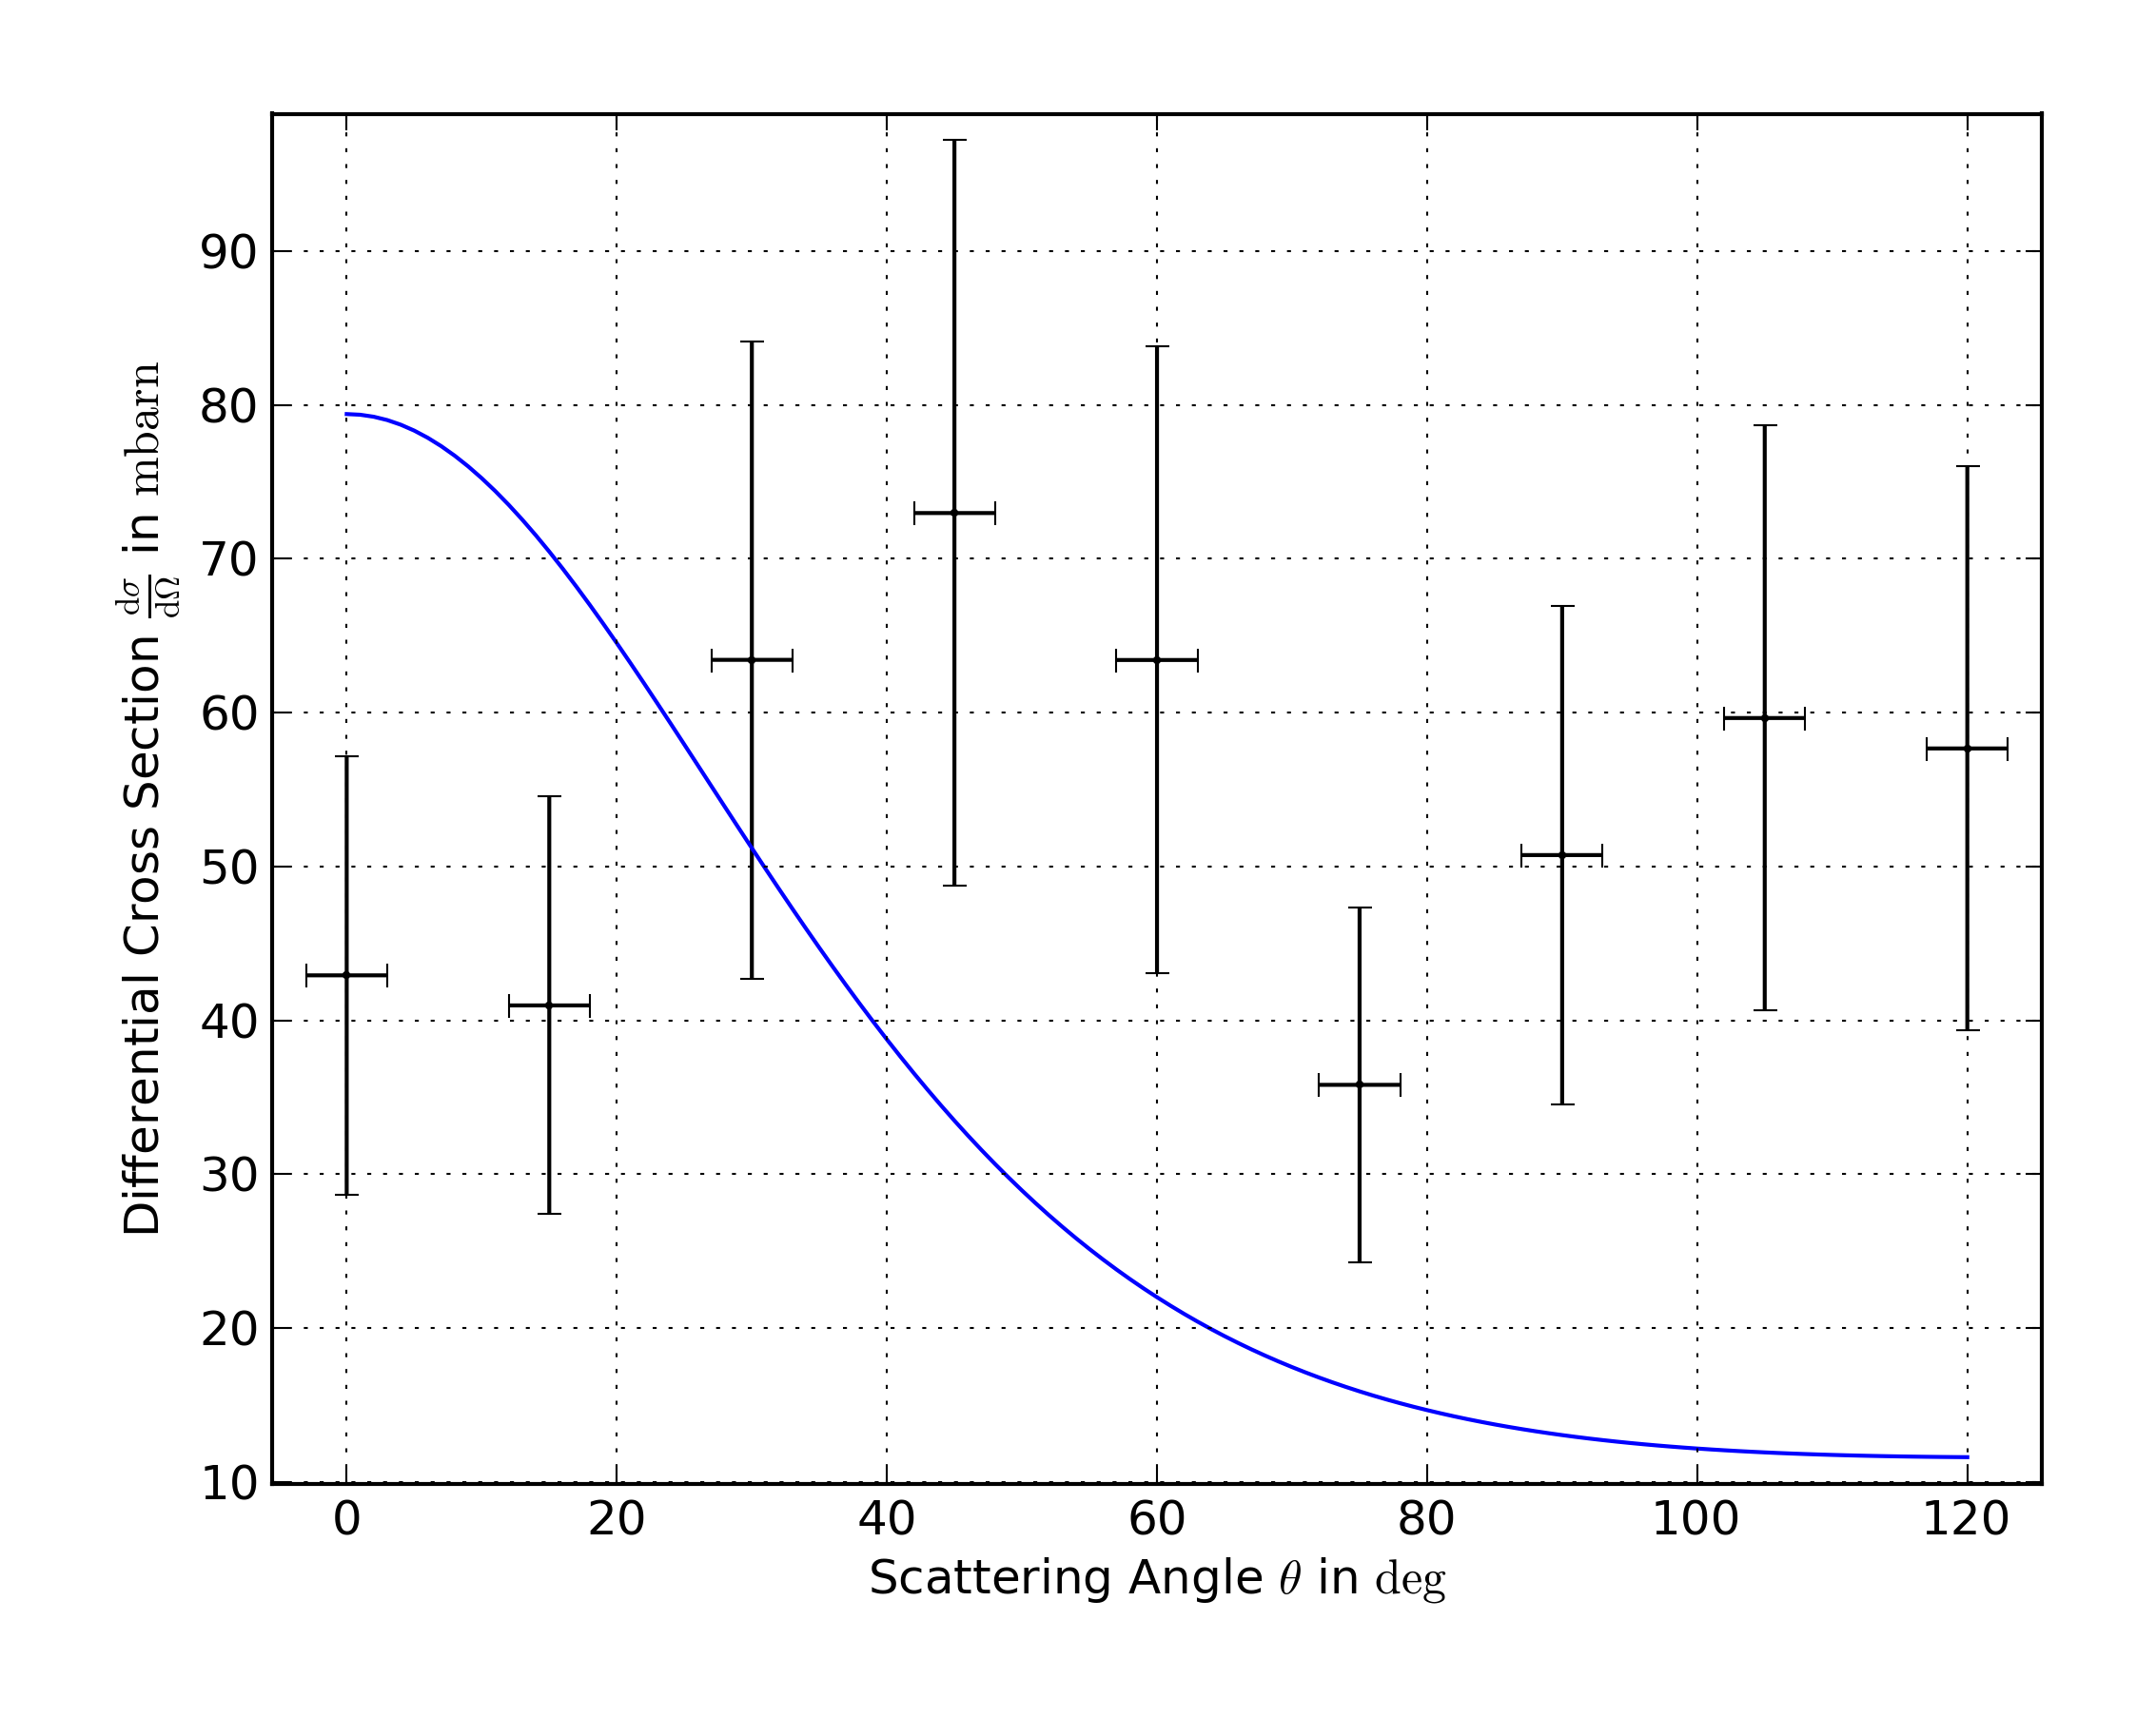
\includegraphics[width=\textwidth]{plots/cross.png}
  \caption{Comparison between measured cross section and theoretical cross
  section. We have estimated the uncertainty of the angle
  $s_\theta=3\degree$ from the setup equipment.}
  \label{fig:cross}
\end{figure}

With (\ref{eq:dcs}) we can finally calculate the differential cross section.
Table \ref{tab:cross} summaries this calculation. Figure \ref{fig:cross}
shows the
calculated values and the values theoretically expected from the
\person{Klein Nishina} formula. It is clearly visible that our values have the
correct order of magnitude. Sadly the standard deviations are rather large and
the values scatter around the expected values.

\subsection{Discussion of Errors}
The calibration fits (figure \ref{fig:calibNaJ} and \ref{fig:calibPVC}) and
the comparison of measured differential cross section and \kleinn formula
in figure \ref{fig:cross} needs some discussion of errors. 

The great $\chi^2/\mathrm{ndf}$ in the calibration fits could have
several reason.
\begin{itemize}
  \item The scintillation process might not be as linear as we supposed.
  The photons might not be totally absorbed in the NaI scintillator. That
  means that they did not deport all their energy. There could be other
  interactions and absorptions inside the scintillator which we do not know.
  
  \item The other group in our room need absolute darkness. To ensure that
  the light from our equipment did not spoil their experiment, they covered
  our rack with a black blanket. The blanked might have turned the delay and
  amplification setting.

  \item All parts of the equipment have probably temperature dependent
  properties which might have changes over time.

  \item The digital pulses from the TSCAs were rather short compared to the
  analogous signals. This means that even with perfectly delayed signals the
  linear gate will cut parts of the analogous signals. This clearly affects
  our measurement.
\end{itemize}

The measured differential cross section scatters randomly around the
theoretical values. Of course the possible sources of errors from above apply here as
well. The measurement could be improved by prolonged
measurement durations, because the peaks had only about 5 counts!
An other source of errors is the assumption that the individual cross
sections of the electrons do not overlap. Probably the greatest uncertainty
factors are the values of $\mu$ and $\varepsilon$. These could be reduced by
finding more readable sources.

